%%%%%%%%%%%%%%%%%%%%%%%%%%%%%%%%%%%%%%%%%%%%%%%%%%%%%%%%%%%%%%%%%%%%%%
% Overleaf (WriteLaTeX) Example: Molecular Chemistry Presentation
%
% Source: http://www.overleaf.com
%
% In these slides we show how Overleaf can be used with standard 
% chemistry packages to easily create professional presentations.
% 
% Feel free to distribute this example, but please keep the referral
% to overleaf.com
% 
%%%%%%%%%%%%%%%%%%%%%%%%%%%%%%%%%%%%%%%%%%%%%%%%%%%%%%%%%%%%%%%%%%%%%%
% How to use Overleaf: 
%
% You edit the source code here on the left, and the preview on the
% right shows you the result within a few seconds.
%
% Bookmark this page and share the URL with your co-authors. They can
% edit at the same time!
%
% You can upload figures, bibliographies, custom classes and
% styles using the files menu.
%
% If you're new to LaTeX, the wikibook is a great place to start:
% http://en.wikibooks.org/wiki/LaTeX
%
%%%%%%%%%%%%%%%%%%%%%%%%%%%%%%%%%%%%%%%%%%%%%%%%%%%%%%%%%%%%%%%%%%%%%%

\documentclass[xcolor=dvipsnames]{beamer}

\usetheme{Madrid}
\useoutertheme{split} % Alternatively: miniframes, infolines, split
\useinnertheme{circles}

%%%%%%%%%%
% Giorgio Morandi #colors_1
\definecolor{color0}{HTML}{372639}
\definecolor{color1}{HTML}{C2A4C0}
\definecolor{color2}{HTML}{816288}
\definecolor{color3}{HTML}{C6926C}
\definecolor{color4}{HTML}{D5BEA9}
\definecolor{color5}{HTML}{DBCAD3}
%%%%%%%%%%

%%%%%%%%%%
\setbeamercolor{normal text}{bg = color5!25, fg = color0}
%\setbeamercolor{alerted text}{bg = color5, fg = color1}
%\setbeamercolor{example text}{bg = color5, fg = color1!50!color0}

\setbeamercolor{palette primary}{bg = color3, fg = color5!50}
%\setbeamercolor{palette secondary}{bg = color1, fg = color5}
%\setbeamercolor{palette tertiary}{bg = color4, fg = color5}

\setbeamercolor{palette quaternary}{bg = color2!50, fg = color0!75}

\setbeamercolor{structure}{bg = color5!50, fg = color4} % itemize, enumerate, etc

\setbeamercolor{section in toc}{bg = color5!50, fg = color1} % TOC sections

% Override palette coloring with secondary
\setbeamercolor{subsection in head/foot}{bg = color3!50, fg = color2}
% For more themes, color themes and font themes, see:
% http://deic.uab.es/~iblanes/beamer_gallery/index_by_theme.html
%%%%%%%%%%

%%%%%%%%%%
\mode<presentation>
{
  \usetheme{Madrid}       % or try default, Darmstadt, Warsaw, ...
  \usecolortheme{default} % or try albatross, beaver, crane, ...
  \usefonttheme{serif}    % or try default, structurebold, ...
  \setbeamertemplate{navigation symbols}{}
  \setbeamertemplate{caption}[numbered]
} 

\usepackage[english, french]{babel}
\usepackage[utf8x]{inputenc}
\usepackage{chemfig}
\usepackage[version = 3]{mhchem}

% On Overleaf, these lines give you sharper preview images.
% You might want to `comment them out before you export, though.
\usepackage{pgfpages}
\pgfpagesuselayout{resize to}[%
  physical paper width = 8in, physical paper height = 6in]
  
% Here's where the presentation starts, with the info for the title slide
\title[SYSTÈMES INTELLIGENTS]{\textsc{SYSTÈMES INTELLIGENTS \\\normalsize{POUR LA TRANSMISSION DES \\HUMANITÉS NUMÉRIQUES \\ET POUR LA RECHERCHE EN SANTÉ}}}
\institute{\large{\texttt{LECLA}}}
\author{Directeur de thèse (HDR) : Thibaud HULIN
\\Présentateur : Hao ZHANG}

\usepackage{datetime}
\newdate{date}{25}{6}{2021}
\date{\displaydate{date}}
%\date{11 novembre 2018}

\logo{\includegraphics[height = 20mm]{images/logo.png}}

\setbeamersize{text margin left = 0.25in, text margin right = 0.25in}

\usepackage{ragged2e}
\renewcommand{\raggedright}{\leftskip=0pt \rightskip=0pt plus 0.25in}

\begin{document}

\begin{frame}
	\titlepage
\end{frame}

\section{À propos de moi}

\begin{frame}
	\frametitle{Sommaire}
	\tableofcontents[currentsection]
\end{frame}

\begin{frame}[fragile]
	\frametitle{À propos de moi}
		\begin{block}{Formation}
			\small{
			\begin{itemize}
				\item[$\bullet$]Étudiant de Mastère Spécialisé Smart System \& IoT (Internet of Things) de CY Tech, une grande école administrée par CY Cergy Paris Université
				\item[$\bullet$]Diplôme d'ingénieur de l'ESLIV (École Supérieure d'Ingénieurs Léonard de Vinci) en IBO (Informatique, Big Data et Object Connecté) en option data science
				\item[$\bullet$]Formation de 5 ans de médecine ce qui est équivalente à une licence
				\item[$\bullet$]Participation à un programme d'échange franco-chinois sur la médecine d'urgences
				\item[$\bullet$]Note de 3e année du cycle ingénieur : 14,92 ; note de stage : 16,72 ; TOEIC 800; DALF Science C1 (français)  
			\end{itemize}}
		\end{block}
\vspace{1.2cm}
\end{frame}

\begin{frame}[fragile]
\frametitle{À propos de moi}
\begin{block}{Expérience}
	\small{
	\begin{itemize}
		\item[$\bullet$]Bonne maîtrise des langages de programmation (Python, R, JavaScript, etc.) et des bases de données (SQL, MongeDB, etc.)
		\item[$\bullet$]Bonne connaissance du domaine de Data Science, Machine Learning, TAL(Traitement automatique des Langues) et IoT
		\item[$\bullet$]Participation aux projets d'IA comme le traitement d'image et de langage
		\item[$\bullet$]Plus d'un an d'expérience dans une entreprise pharmaceutique en étudiant de nouveaux médicaments et leur résultat d'essai clinique
		\item[$\bullet$]Êtes curieux et ouvert d'esprit à propos des humanités en général
	\end{itemize}}
\end{block}
\vspace{1.1cm}
\end{frame}

\section{Humanités Numériques (HN)}

\begin{frame}
\frametitle{Sommaire}
\tableofcontents[currentsection]
\end{frame}

\begin{frame}{Humanités Numériques (HN)}
\begin{columns}
	\column{0.6\textwidth}
	\small{
		\begin{itemize}
		\item[$\bullet$]Les Humanités Numériques (HN) forment un socle de partage, d'étude et de formation à des concepts ou à des compétences de haut niveau (dont dépendent les autres compétences), pour apprendre avec les technologies numériques.
		\item[$\bullet$]Avec les humanités numériques et les méthodes d'intelligence artificielle, la machine peut facilement reconnaître les textes manuscrits dans les archives, rechercher l'information et représenter des données via des graphes.
	\end{itemize}}
	\column{0.4\textwidth}
	\begin{figure}[ht]
		\begin{center}
			\includegraphics[width=\textwidth]{./images/Humanites_Numeriques.JPG}
			\vspace{1.5cm}
		\end{center}
	\end{figure}
\end{columns}
\end{frame}

\section{À propos du projet}

\begin{frame}
\frametitle{Sommaire}
\tableofcontents[currentsection]
\end{frame}

\subsection{Environnement et partenaires}
\begin{frame}[fragile]
\centering
\frametitle{Environnement et partenaires}
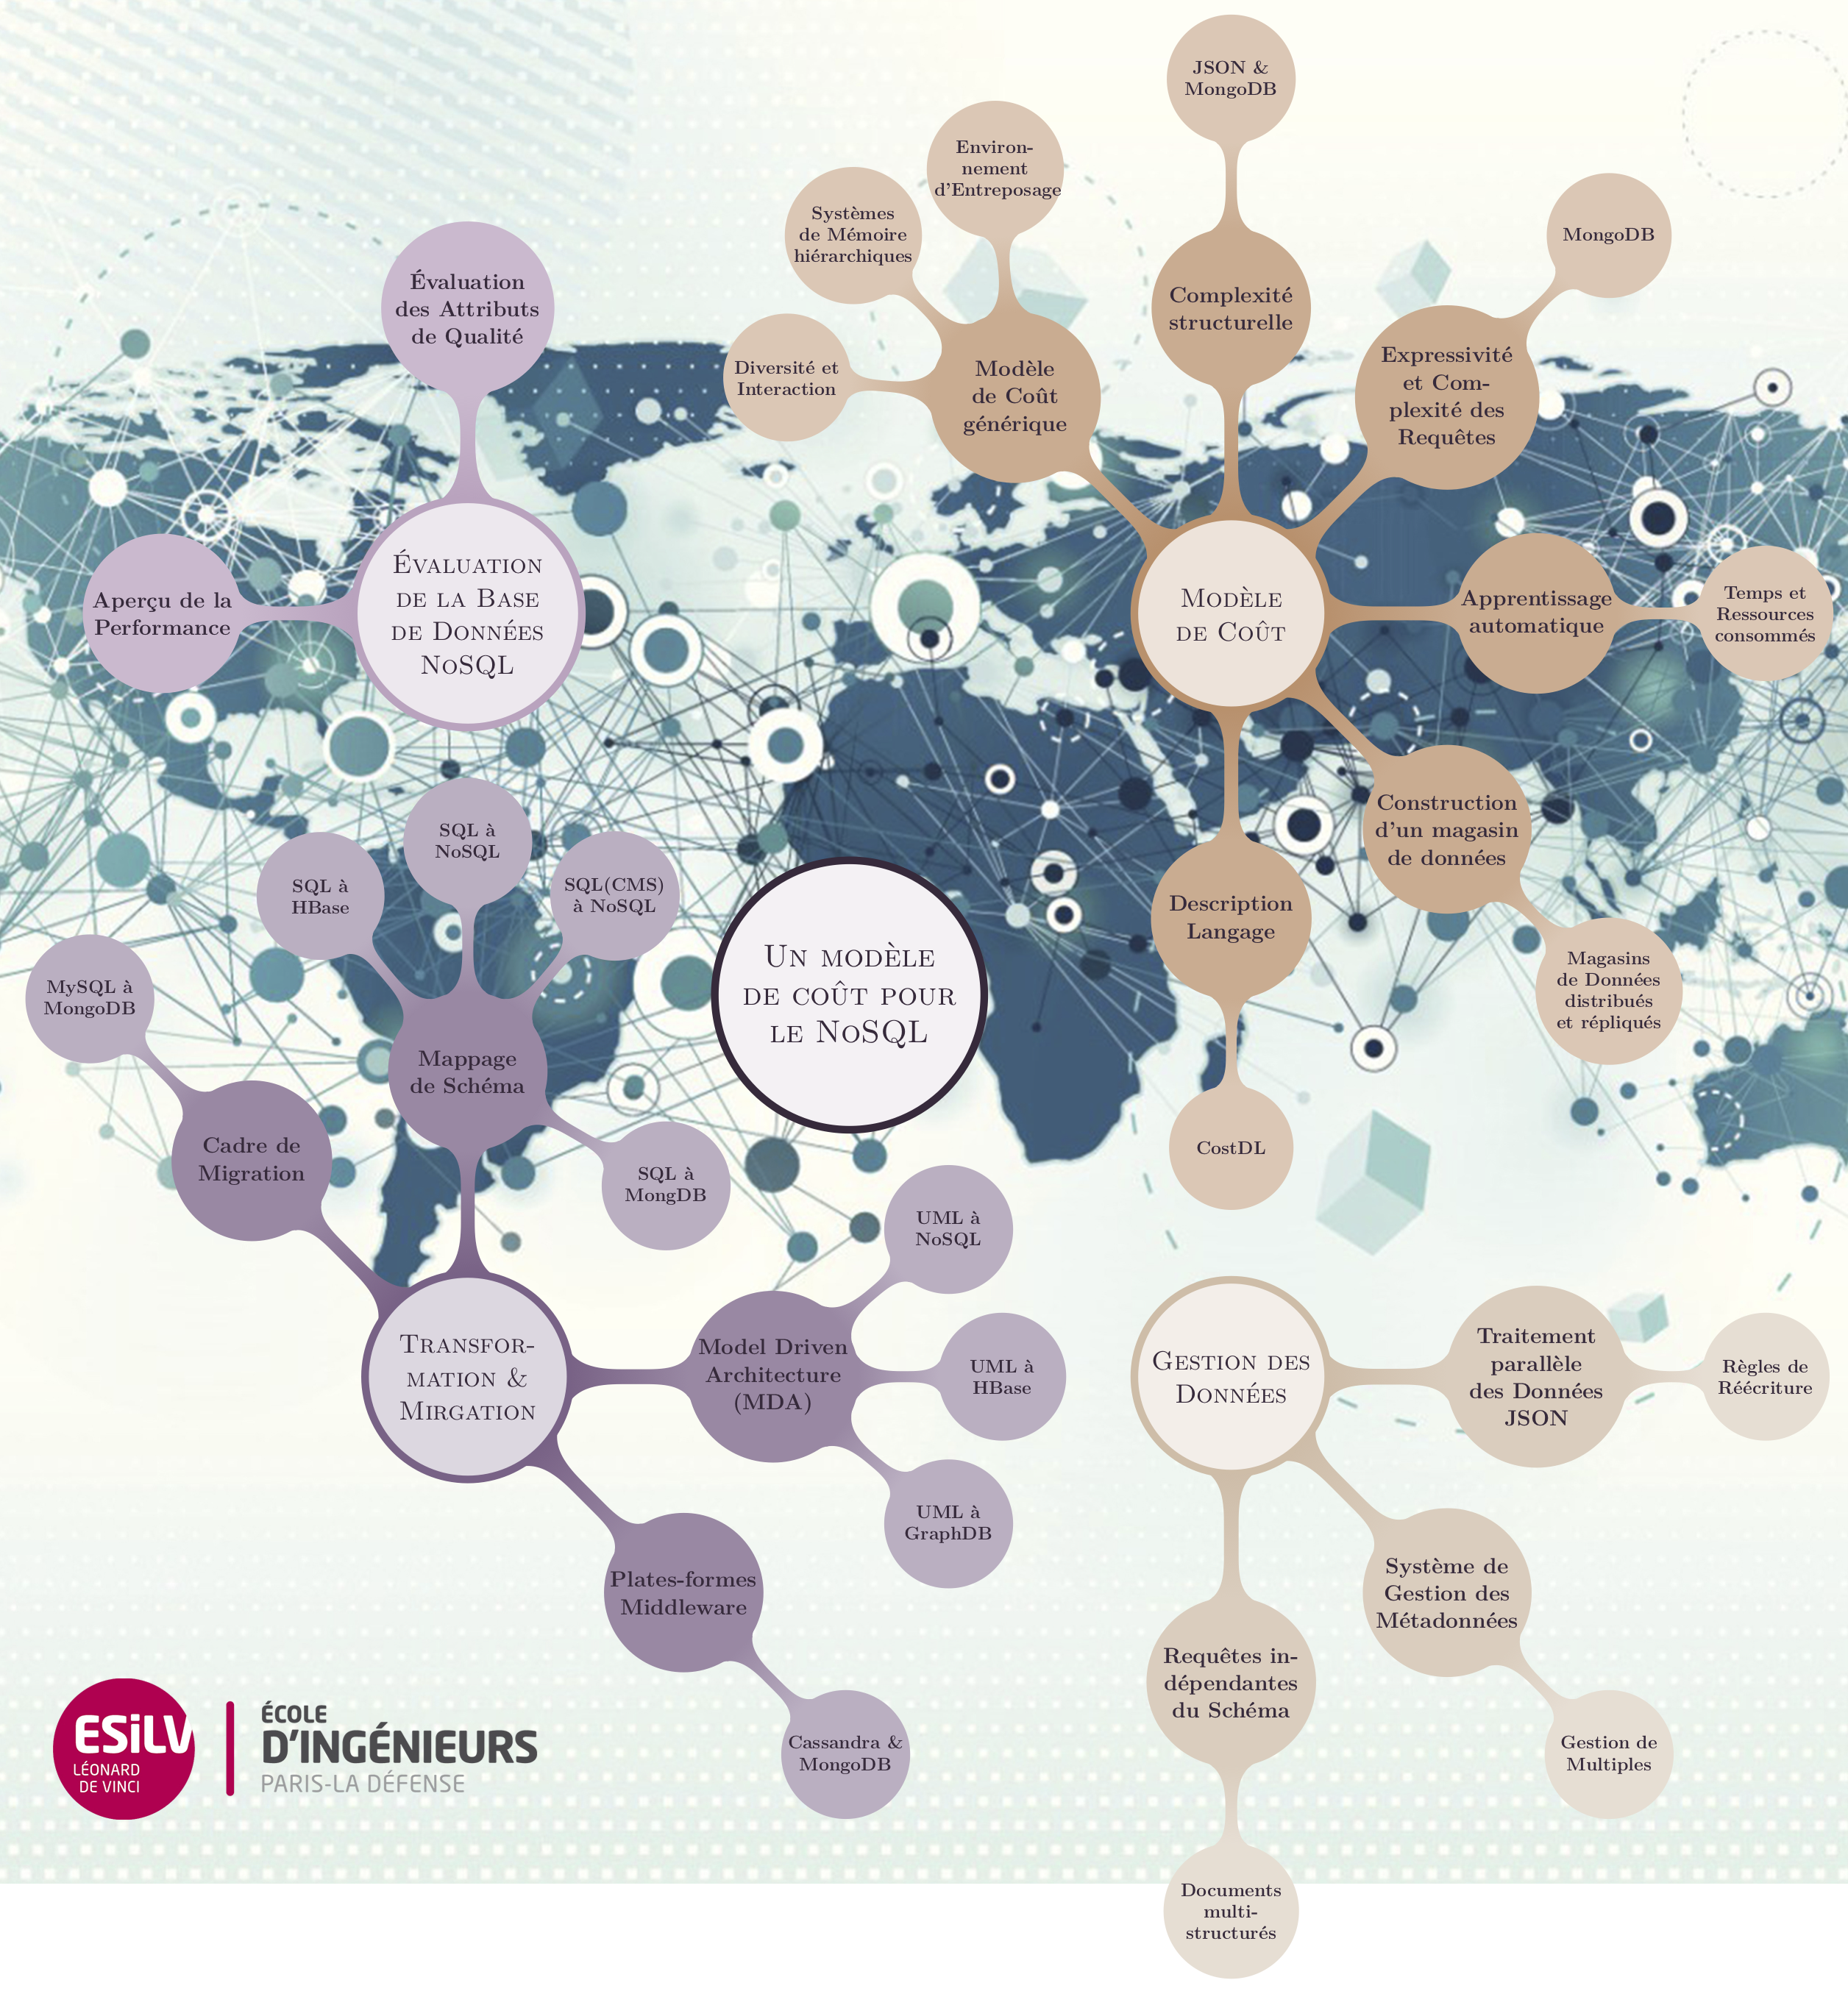
\includegraphics[height = 6.7cm]{images/mindmap.png}
\end{frame}

\subsection{Objectifs de la recherche en IA
}
\begin{frame}[fragile]
\frametitle{Objectifs de la recherche en IA
}
\begin{columns}
	\column{0.475\textwidth}
	\begin{block}{Les données sont :}
		\small{
		\begin{itemize}
			\item[$\bullet$]les scénarios de cours produits par les enseignants
			\item[$\bullet$]les fonds d'archives numérisés, à valoriser en pédagogie, et pour les chercheurs (notamment du pôle thématique LLC)
		\end{itemize}}
	\end{block}
\vspace{4cm}
	\column{0.475\textwidth}
	\begin{block}{L'IA :}
		\small{
		\begin{itemize}
		\item[$\bullet$]suggère des ressources pertinentes pour les enseignants
		\item[$\bullet$]permet de visualiser les données pour les chercheurs en HN, voire en pédagogie
		\item[$\bullet$]fournit d'autres services comme : reconnaissance du texte dans les manuscrits, système de recommandation, etc.
		\end{itemize}}
	\end{block}
\vspace{2.5cm}
\end{columns}
\end{frame}

\subsection{Démarche globale}
\begin{frame}[fragile]
\frametitle{Démarche globale}
\begin{block}{Démarche globale 1 / 2}
	\begin{itemize}
		\item[$\bullet$]Cartographier le champ grâce à la mobilisation d'experts du domaine. (Ce travail a déjà commencé.)
		\item[$\bullet$]Collecter les données d'expérience pédagogiques sur une plateforme dédiée.
		\item[$\bullet$]Concevoir des services en comparant des cas d'utilisation en santé et en humanités. (ex. : classification, croisement des données, regroupements, etc.)
	\end{itemize}
\end{block}
\vspace{2cm}
\end{frame}

\begin{frame}[fragile]
\frametitle{Démarche globale}
\begin{block}{Démarche globale 2 / 2}
	\begin{itemize}
		\item[$\bullet$]Développer des services intelligents pour la recherche d'information, la visualisation et l'analyse des données.
		\item[$\bullet$]Évaluer les usages (analyse des traces, mouvements oculaires, enquêtes...). La recherche de eye-tracking peut être en collaboration avec l'équipe ERCOS de ELLIADD.
		\item[$\bullet$]Observer les pratiques d'enseignement et communiquer sur le projet.
	\end{itemize}
\end{block}
\vspace{2cm}
\end{frame}

\subsection{Web sémantique et intelligence artificielle}
\begin{frame}{Utiliser les technologies du web sémantique pour construire des services intelligents}
\begin{columns}
	\column{1.05\textwidth}
	\small{
	\begin{itemize}
	\item[$\bullet$]Le W3C est un organisme de standardisation à but non lucratif pour faciliter l'échange de données sur le Web. La co-directrice de thèse, experte en informatique et en sciences cognitives, Mme McGuiness en fait partie et y contribue.
	\end{itemize}}
	\vspace{-0.4cm}
\end{columns}
	\begin{columns}
	\column{0.65\textwidth}
	\small{
	\begin{itemize}
		\item[$\bullet$]Le Web sémantique est une extension du Web standardisé par le W3C. Ses standards encouragent l'utilisation de formats de données et de protocoles d'échange normés sur le Web, en s'appuyant sur le modèle Resource Description Framework (RDF) qui est la technologie centrale du Web sémantique. 
	\end{itemize}}
	\vspace{3cm}
	\column{0.375\textwidth}
	\begin{figure}[ht]
		\begin{center}
			\includegraphics[width=\textwidth]{./images/Semantic_Web.png}
		\end{center}
	\end{figure}
	\vspace{4cm}
\end{columns}
\end{frame}

\begin{frame}[fragile]
\frametitle{Web sémantique et intelligence artificielle}
\begin{columns}
	\column{0.475\textwidth}
	\begin{block}{Rôle du Web Sémantique}
		\begin{itemize}
			\item[$\bullet$]modéliser le domaine d'un discours
			\item[$\bullet$]identifier les éléments (terminologie), les relations, notamment entre classes et individus
			\item[$\bullet$] construire une ontologie (base de connaissance)
		\end{itemize}
	\end{block}
	\column{0.475\textwidth}
	\begin{block}{Rôle de l'IA grâce au WS}
		\begin{itemize}
			\item[$\bullet$]trouver des régularités
			\item[$\bullet$]calculer des proximités entre ressources
			\item[$\bullet$]construire automatiquement une ontologie à partir d'un corpus de textes (via une intelligence artificielle de type connexioniste)
		\end{itemize}
	\end{block}
\end{columns}
\end{frame}

\begin{frame}[fragile]
\frametitle{Exemple d'ontologie}
\includegraphics[height = 6.7cm]{images/Ontologie_2.png}
\end{frame}

\subsection{Exemple d'ontologie}
\begin{frame}[fragile]
\frametitle{Exemple d'ontologie}
	\includegraphics[height = 6.7cm]{images/Ontologie_1.png}
\end{frame}

\section{Conclusion}
\begin{frame}
\frametitle{Sommaire}
\tableofcontents[currentsection]
\end{frame}

\begin{frame}[fragile]
\frametitle{Conclusion}
\begin{block}{Les apports de la thèse pour l'école doctorale sont :}
	\small{
		\begin{itemize}
			\item[$\bullet$]Valoriser des corpus issus de la \textbf{littérature} (ex. : le fond Queneau de l'UB), dans le cadre de séances de médiation des savoirs ou de médiation culturelles (fonds photographiques);
			\item[$\bullet$]Renouveler l'analyse \textbf{linguistique} de ces corpus grâce à la sémantisation des données issues des textes (via une ontologie comme Wordnet).
			\item[$\bullet$]L'ontologie permettra aussi de travailler sur les traductions des textes en différentes langues, ex. : les \textbf{traductions} des textes de Queneau.
			\item[$\bullet$]Ainsi, toutes les grandes disciplines de l'école doctorale seront conviées pour participer au projet sur \textbf{l'Émancipation du Pôle Thématique} Lettres, Langues et Communication.
	\end{itemize}}
\end{block}
\vspace{3cm}
\end{frame}

\begin{frame}[fragile]
	\frametitle{Conclusion}
	\begin{block}{Pour conclure...}
		\small{
	\begin{itemize}
		\item[$\bullet$]Une occasion unique de collaboration internationale avec celles et ceux qui font le web
		\item[$\bullet$]Cette thèse s'inscrira dans un environnement très stimulant, impliquant de nombreuses disciplines : toutes celles enseignées de l'école au lycée, en SHS (linguistique, Information-Communication, littérature, langues…), en informatique, en science cognitive et en santé.
		\item[$\bullet$]Des retours sont attendus pour tous les participants de laboratoires différents, via le programme Émancipation du Pothem LLC.
		\item[$\bullet$]Mon dossier a été sélectionné par l'Institut Polytechnique de Rensselaer (état de NY) et par M. HULIN grâce à mes compétences informatiques, en langues et en santé, mon expérience en IA et mon niveau d'ingénieur.
	\end{itemize}}
\end{block}
\end{frame}

\begin{frame}[fragile]
\frametitle{Merci !}
\begin{block}{Quelques références}
	\tiny{
		\begin{itemize}
\item[$\bullet$]Ageeva, N. A., Shapoval, G. N., Vlasova, V. N., Kartashova, E. A., Safronenko, A. V., \& \item[$\bullet$]Sidorenko, Y. A. (2019). High level of legal awareness formation in medical students. Way from competencies to competence. Espacios, 40(9), 11.
\item[$\bullet$]Berners-Lee, Tim, James Hendler, et Ora Lassila. « The semantic web ». Scientific american 284, no 5 (2001): 34‑43.
\item[$\bullet$]Hulin, T. (2016). Vers une plateforme sémantique pour l’enseignement des sciences et de la culture numérique. Tréma, 42, 37‑49.
\item[$\bullet$]McCusker, J., Rashid, S. M., Agu, N., Bennett, K. P., \& McGuinness, D. L. (2018). The Whyis Knowledge Graph Framework in Action. International Semantic Web Conference (P\&D/Industry/BlueSky).
\item[$\bullet$]Roxin, I., \& Tajariol, F. (2019). Information, communication et humanités numériques. Enjeux et défis pour un enrichissement épistémologique. Actes du colloque « HumaNum » – I Roxin et all.
\item[$\bullet$]Hulin, T., Collet, L. \& Rémond, É. (2021). Les enjeux de la formation de formateurs aux humanités numériques. In F. Paquienséguy \& N. Pélissier, Questionner les humanités numériques : Positions et propositions des SIC (SFSIC et CPdirsic, p. 257‑273). CPDirSIC.
	\end{itemize}}
\end{block}
\end{frame}

\end{document}